\subsection{Test}
Testing of the FSMd implementation of the vending machine controller is done with modelsim.
In order to insure that the design is working as intended, it should be verified that
all of the requirements from the specification are met. 
This can be done with the following test sequence.
\begin{enumerate}
    \item Assert \textbf{coin2}, verify that the controller adds 2 to \textbf{sum} and waits for \textbf{coin2} to be deasserted.
    \item Assert \textbf{coin5}, verify that the controller adds 5 to \textbf{sum} and waits for \textbf{coin5} to be deasserted.
    \item Assert \textbf{buy}, verify that the controller can compare \textbf{sum} and \textbf{price} correctly and assert either \textbf{alarm} or \textbf{release\_can}.
    \item Assert \textbf{reset}, verify that the controller resets it's state and \textbf{sum}.
\end{enumerate}
It can also be verified that the controller shows the correct numbers on the 7-segment display using modelsim, however this is much easier to do 
visually using the Basys2 board. \\

Since operation of the machine assumes that the \textbf{sum} will never exceed the maximum value the machine can handle, this will not be tested.
Should it happen, it would cause overflow because of the datapath implementation. \\

To test the FSMd implementation, the following .do file seen in listing \ref{fsmd_do} was used. The result of the simulation can be seen 
in figure \ref{fsmd_sim}.

\lstinputlisting[caption={.do file for testing the vending machine FSMd}, label={fsmd_do}]{../project1/src/controllertest.do}

\begin{figure}
    \center
    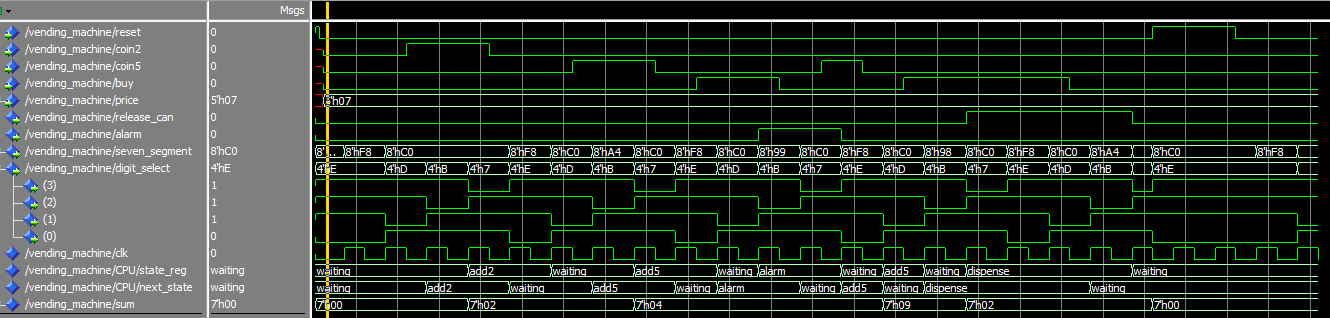
\includegraphics[scale=0.5]{pictures/FSMd_test.png}
    \caption{Modelsim simulation of the vending machine FSMd using the .do file from listing \ref{fsmd_do} }
    \label{fsmd_sim}
\end{figure}

The timing diagram in figure \ref{fsmd_sim} shows that the vending machine controller correctly multiplexes the display,
accepts input and waits for inputs to be deasserted before continuing, and can perform a transaction provided that
the \textbf{sum} is larger than the price. It can also be seen that \textbf{release\_can} is asserted for as long
as \textbf{buy} is pressed and that \textbf{reset} works as specified.
